% !Tex root = main.tex
%-----------------------------------------------------------------------------------------------------------------------------------------------%
%	The MIT License (MIT)
%
%	Copyright (c) 2019 Jan Küster
%
%	Permission is hereby granted, free of charge, to any person obtaining a copy
%	of this software and associated documentation files (the "Software"), to deal
%	in the Software without restriction, including without limitation the rights
%	to use, copy, modify, merge, publish, distribute, sublicense, and/or sell
%	copies of the Software, and to permit persons to whom the Software is
%	furnished to do so, subject to the following conditions:
%	
%	THE SOFTWARE IS PROVIDED "AS IS", WITHOUT WARRANTY OF ANY KIND, EXPRESS OR
%	IMPLIED, INCLUDING BUT NOT LIMITED TO THE WARRANTIES OF MERCHANTABILITY,
%	FITNESS FOR A PARTICULAR PURPOSE AND NONINFRINGEMENT. IN NO EVENT SHALL THE
%	AUTHORS OR COPYRIGHT HOLDERS BE LIABLE FOR ANY CLAIM, DAMAGES OR OTHER
%	LIABILITY, WHETHER IN AN ACTION OF CONTRACT, TORT OR OTHERWISE, ARISING FROM,
%	OUT OF OR IN CONNECTION WITH THE SOFTWARE OR THE USE OR OTHER DEALINGS IN
%	THE SOFTWARE.
%	
%
%-----------------------------------------------------------------------------------------------------------------------------------------------%


%============================================================================%
%
%	DOCUMENT DEFINITION
%
%============================================================================%

%we use article class because we want to fully customize the page and don't use a cv template
\documentclass[10pt,A4]{article}	


%----------------------------------------------------------------------------------------
%	ENCODING
%----------------------------------------------------------------------------------------

% we use utf8 since we want to build from any machine
\usepackage[utf8]{inputenc}		

%----------------------------------------------------------------------------------------
%	LOGIC
%----------------------------------------------------------------------------------------

% provides \isempty test
\usepackage{xstring, xifthen}

%----------------------------------------------------------------------------------------
%	FONT BASICS
%----------------------------------------------------------------------------------------

% some tex-live fonts - choose your own

%\usepackage[defaultsans]{droidsans}
%\usepackage[default]{comfortaa}
%\usepackage{cmbright}
\usepackage[default]{raleway}
%\usepackage{fetamont}
%\usepackage[default]{gillius}
%\usepackage[light,math]{iwona}
%\usepackage[thin]{roboto} 

% set font default
\renewcommand*\familydefault{\sfdefault} 	
\usepackage[T1]{fontenc}

% more font size definitions
\usepackage{moresize}

%----------------------------------------------------------------------------------------
%	FONT AWESOME ICONS
%---------------------------------------------------------------------------------------- 

% include the fontawesome icon set
\usepackage{fontawesome}

% use to vertically center content
% credits to: http://tex.stackexchange.com/questions/7219/how-to-vertically-center-two-images-next-to-each-other
\newcommand{\vcenteredinclude}[1]{\begingroup
\setbox0=\hbox{\includegraphics{#1}}%
\parbox{\wd0}{\box0}\endgroup}

% use to vertically center content
% credits to: http://tex.stackexchange.com/questions/7219/how-to-vertically-center-two-images-next-to-each-other
\newcommand*{\vcenteredhbox}[1]{\begingroup
\setbox0=\hbox{#1}\parbox{\wd0}{\box0}\endgroup}

% icon shortcut
\newcommand{\icon}[3] { 							
	\makebox(#2, #2){\textcolor{maincol}{\csname fa#1\endcsname}}
}	

% icon with text shortcut
\newcommand{\icontext}[4]{ 						
	\vcenteredhbox{\icon{#1}{#2}{#3}}  \hspace{2pt}  \parbox{0.9\mpwidth}{\textcolor{#4}{#3}}
}

% icon with website url
\newcommand{\iconhref}[5]{ 						
    \vcenteredhbox{\icon{#1}{#2}{#5}}  \hspace{2pt} \href{#4}{\textcolor{#5}{#3}}
}

% icon with email link
\newcommand{\iconemail}[5]{ 						
    \vcenteredhbox{\icon{#1}{#2}{#5}}  \hspace{2pt} \href{mailto:#4}{\textcolor{#5}{#3}}
}

%----------------------------------------------------------------------------------------
%	PAGE LAYOUT  DEFINITIONS
%----------------------------------------------------------------------------------------

% page outer frames (debug-only)
% \usepackage{showframe}		
%package to display URLs as such in the pdf
%\usepackage{hyperref}

% we use paracol to display breakable two columns
\usepackage{paracol}

% define page styles using geometry
\usepackage[a4paper]{geometry}

% remove all possible margins
\geometry{top=1cm, bottom=1cm, left=1cm, right=1cm}

\usepackage{fancyhdr}
\pagestyle{empty}

% space between header and content
% \setlength{\headheight}{0pt}

% indentation is zero
\setlength{\parindent}{0mm}

%----------------------------------------------------------------------------------------
%	TABLE /ARRAY DEFINITIONS
%---------------------------------------------------------------------------------------- 

% extended aligning of tabular cells
\usepackage{array}

% custom column right-align with fixed width
% use like p{size} but via x{size}
\newcolumntype{x}[1]{%
>{\raggedleft\hspace{0pt}}p{#1}}%


%----------------------------------------------------------------------------------------
%	GRAPHICS DEFINITIONS
%---------------------------------------------------------------------------------------- 

%for header image
\usepackage{graphicx}

% use this for floating figures
% \usepackage{wrapfig}
% \usepackage{float}
% \floatstyle{boxed} 
% \restylefloat{figure}

%for drawing graphics		
\usepackage{tikz}				
\usetikzlibrary{shapes, backgrounds,mindmap, trees}

%----------------------------------------------------------------------------------------
%	Color DEFINITIONS
%---------------------------------------------------------------------------------------- 
\usepackage{transparent}
\usepackage{color}

% primary color
\definecolor{maincol}{RGB}{ 225, 0, 0 }

% accent color, secondary
% \definecolor{accentcol}{RGB}{ 250, 150, 10 }

% dark color
\definecolor{darkcol}{RGB}{ 70, 70, 70 }

% light color
\definecolor{lightcol}{RGB}{245,245,245}


% Package for links, must be the last package used
\usepackage[hidelinks]{hyperref}

% returns minipage width minus two times \fboxsep
% to keep padding included in width calculations
% can also be used for other boxes / environments
\newcommand{\mpwidth}{\linewidth-\fboxsep-\fboxsep}
	


%============================================================================%
%
%	CV COMMANDS
%
%============================================================================%

%----------------------------------------------------------------------------------------
%	 CV LIST
%----------------------------------------------------------------------------------------

% renders a standard latex list but abstracts away the environment definition (begin/end)
\newcommand{\cvlist}[1] {
	\begin{itemize}{#1}\end{itemize}
}

%----------------------------------------------------------------------------------------
%	 CV TEXT
%----------------------------------------------------------------------------------------

% base class to wrap any text based stuff here. Renders like a paragraph.
% Allows complex commands to be passed, too.
% param 1: *any
\newcommand{\cvtext}[1] {
	\begin{tabular*}{1\mpwidth}{p{0.98\mpwidth}}
		\parbox{1\mpwidth}{#1}
	\end{tabular*}
}

%----------------------------------------------------------------------------------------
%	CV SECTION
%----------------------------------------------------------------------------------------

% Renders a a CV section headline with a nice underline in main color.
% param 1: section title
\newcommand{\cvsection}[1] {
	\vspace{14pt}
	\cvtext{
		\textbf{\LARGE{\textcolor{darkcol}{\uppercase{#1}}}}\\[-4pt]
		\textcolor{maincol}{ \rule{0.1\textwidth}{2pt} } \\
	}
}

%----------------------------------------------------------------------------------------
%	META SKILL
%----------------------------------------------------------------------------------------

% Renders a progress-bar to indicate a certain skill in percent.
% param 1: name of the skill / tech / etc.
% param 2: level (for example in years)
% param 3: percent, values range from 0 to 1
\newcommand{\cvskill}[3] {
	\begin{tabular*}{1\mpwidth}{p{0.72\mpwidth}  r}
 		\textcolor{black}{\textbf{#1}} & \textcolor{maincol}{#2}\\
	\end{tabular*}%
	
	\hspace{4pt}
	\begin{tikzpicture}[scale=1,rounded corners=2pt,very thin]
		\fill [lightcol] (0,0) rectangle (1\mpwidth, 0.15);
		\fill [maincol] (0,0) rectangle (#3\mpwidth, 0.15);
  	\end{tikzpicture}%
}


%----------------------------------------------------------------------------------------
%	 CV EVENT
%----------------------------------------------------------------------------------------

% Renders a table and a paragraph (cvtext) wrapped in a parbox (to ensure minimum content
% is glued together when a pagebreak appears).
% Additional Information can be passed in text or list form (or other environments).
% the work you did
% param 1: time-frame i.e. Sep 14 - Jan 15 etc.
% param 2:	 event name (job position etc.)
% param 3: Customer, Employer, Industry
% param 4: Short description
% param 5: work done (optional)
% param 6: technologies include (optional)
% param 7: achievements (optional)
\newcommand{\cvevent}[7] {
	
	% we wrap this part in a parbox, so title and description are not separated on a pagebreak
	% if you need more control on page breaks, remove the parbox
	\parbox{\mpwidth}{
		\begin{tabular*}{1\mpwidth}{p{0.72\mpwidth}  r}
	 		\textcolor{black}{\textbf{#2}} & \colorbox{maincol}{\makebox[0.25\mpwidth]{\textcolor{white}{#1}}} \\
			\textcolor{maincol}{\textbf{#3}} & \\
		\end{tabular*}\\[8pt]
	
		\ifthenelse{\isempty{#4}}{}{
			\cvtext{#4}\\
		}
	}

	\ifthenelse{\isempty{#5}}{}{
		\vspace{9pt}
		{#5}
	}

	\ifthenelse{\isempty{#6}}{}{
		\vspace{9pt}
		\cvtext{\textbf{Tecnologías:}}\\
		{#6}
	}

	\ifthenelse{\isempty{#7}}{}{
		\vspace{9pt}
		\cvtext{\textbf{Logros:}}\\
		{#7}
	}
	\vspace{14pt}
}

%----------------------------------------------------------------------------------------
%	 CV META EVENT
%----------------------------------------------------------------------------------------

% Renders a CV event on the sidebar
% param 1: title
% param 2: subtitle (optional)
% param 3: customer, employer, etc,. (optional)
% param 4: info text (optional)
\newcommand{\cvmetaevent}[4] {
	\textcolor{maincol} {\cvtext{\textbf{\begin{flushleft}#1\end{flushleft}}}}

	\ifthenelse{\isempty{#2}}{}{
	\textcolor{darkcol} {\cvtext{\textbf{#2}} }
	}

	\ifthenelse{\isempty{#3}}{}{
		\cvtext{{ \textcolor{darkcol} {#3} }}\\
	}

	\cvtext{#4}\\[14pt]
}

%---------------------------------------------------------------------------------------
%	QR CODE
%----------------------------------------------------------------------------------------

% Renders a qrcode image (centered, relative to the parentwidth)
% param 1: percent width, from 0 to 1
\newcommand{\cvqrcode}[1] {
	\begin{center}
		
\includegraphics[width={#1}\mpwidth]{qrcode}
	\end{center}
}
%---------------------------------------------------------------------------------
%UNICOD TROUBLESHOTTING
%------------------------------------------------------------------------------
%\DeclareUnicodeCharacter{200B}{I~AM~HERE!!!!}


%============================================================================%
%
%
%
%	DOCUMENT CONTENT
%
%
%
%============================================================================%
\begin{document}
\columnratio{0.31}
\setlength{\columnsep}{2.2em}
\setlength{\columnseprule}{4pt}
\colseprulecolor{lightcol}
\begin{paracol}{2}
\begin{leftcolumn}
%---------------------------------------------------------------------------------------
%	META IMAGE
%----------------------------------------------------------------------------------------
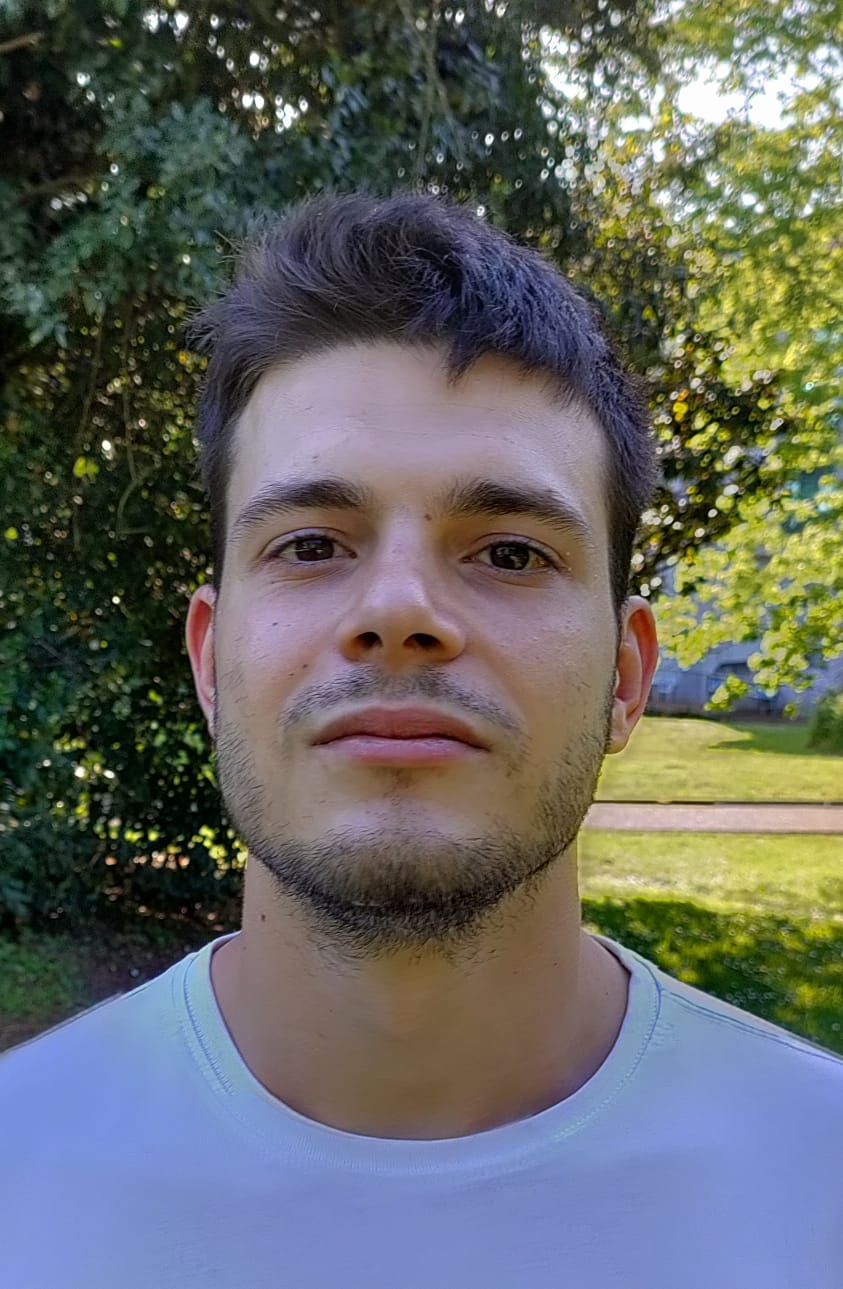
\includegraphics[width=\linewidth]{foto_perfil_buena.jpg}	%trimming relative to image size

%---------------------------------------------------------------------------------------
%	META SKILLS
%----------------------------------------------------------------------------------------
\cvsection{HABILIDADES}

\cvskill{R} {+2 años} {1} \\[-2pt]

\cvskill{LaTeX} {+1 año} {0.75}\\ [-2pt]

\cvskill{Python} {-1 año} {0.5} \\[-2pt]

\cvskill{SQL} {-1 año} {0.5}\\[-2pt]


\vfill\null
\cvsection{CONTACTO}
	
\icontext{MapMarker}{12}{Avda. de Lugo 32 2ºA\\15707 Santiago de Compostela, A Coruña}{black}\\[6pt]
\icontext{MobilePhone}{12}{+34 619 56 09 90}{black}\\[6pt]
\iconemail{Envelope}{12}{diegogasn@outlook.es}{diegogasn@gmail.com}{black}\\[6pt]

\vfill\null
\cvqrcode{0.7}

%---------------------------------------------------------------------------------------
%	EDUCATION
%----------------------------------------------------------------------------------------
\newpage
\cvsection{EDUCACIÓN}

\cvmetaevent
{2019 - 2022}
{Máster Interuniversitario en Técnicas Estadísticas}
{Universidade de Santiago de Compostela - Facultade de Matemáticas}
{Técnicas incluidas:
\cvlist{
\item Análisis e inferencia paramétrica y no paramétrica
\item Optimización
\item Regresión
\item Representación de datos
\item Series de tiempo
\item Aprendizaje estadístico supervisado y no supevisado
\item \textit{Machine learning}
\item Manejo de bases de datos y consultas en ellas}
Buena adaptación a la docencia telemática antes y despues de la pandemia\\
Nota media: 7.6222}

\cvmetaevent
{2014 -2019}
{Grado en Psicología}
{Universidade de Santiago de Compostela - Facultade de Psicología}
{Trabajo de fin de grado acerca de la autentificación de individuos en medios digitales a través del electroencefalograma.\\
Programa Erasmus + en la Univerzita Karlova, Praga.\\
Nota media: 8.025}

\vfill\null
\cvqrcode{0.7}

%---------------------------------------------------------------------------------------
%	CERTIFICATION
%----------------------------------------------------------------------------------------
\newpage
\cvsection{CERTIFICADOS}

\cvmetaevent
{Udemy - Intermediate Python Inmersive Training}
{Noviembre, 22}
{}
{}

\cvmetaevent
{Cambridge CAE C1}
{Marzo, 14}
{}
{}

\cvmetaevent
{TOEFL}
{Marzo, 19}
{}
{Puntuación = 100}

\cvmetaevent
{Cinturón Negro de Judo}
{Noviembre, 18}
{}
{2º DAN}


\cvmetaevent
{Carnet de conducir}
{Noviembre, 14}
{}
{Clase B}


\vfill
\cvqrcode{0.7}

\newpage
\mbox{} % hotfix to place qrcode on the bottom when there are not other elements
\vfill
\cvqrcode{0.7}

\end{leftcolumn}
\begin{rightcolumn}
%---------------------------------------------------------------------------------------
%	TITLE  HEADER
%----------------------------------------------------------------------------------------
\fcolorbox{white}{darkcol}{\begin{minipage}[c][3.5cm][c]{1\mpwidth}
	\begin {center}
		\HUGE{ \textbf{ \textcolor{white}{ \uppercase{ DIEGO GARCIA SANCHEZ } } } } \\[-24pt]
		\textcolor{white}{ \rule{0.1\textwidth}{1.25pt} } \\[4pt]
		\large{ \textcolor{white} {Psicólogo | Técnico estadístico | Analista de datos} }
	\end {center}
\end{minipage}} \\[14pt]
\vspace{-12pt}

%---------------------------------------------------------------------------------------
%	PROFILE
%----------------------------------------------------------------------------------------
\vfill\null
\cvsection{PERFIL}

\cvtext{Graduado como psicólogo, estoy enfocándome en las habilidades adquiridas en mi máster en técnicas estadísticas. Una sólida formación teórica promueve un perfil especializado para el análisis de datos relacionados con la psicología. Otros campos bajo mi alcance incluyen investigación de mercado, análisis sensorial y un interés genuino en llevar las últimas tecnologías al usuario final.

Me destaco por tener una buena intuición de la mente humana y un pensamiento crítico entrenado. Trato de mantener actualizado mi conocimiento del mundo, obtuve una alta puntuación en curiosidad intelectual y apertura a la experiencia. La ética laboral también es una característica comúnmente destacada por los empleadores anteriores.

Altamente motivado para trabajar en equipo, tanto en grandes empresas como en pequeños equipos.


De una vida dedicada al judo aprendí valores como la disciplina, la constancia y el respeto.
}

%---------------------------------------------------------------------------------------
%	WORK EXPERIENCE
%----------------------------------------------------------------------------------------
\vfill\null
\cvsection{EXPERIENCIA LABORAL}

\cvevent
	{Sept 20 - Ahora}
	{Co-fundador | Responsable de datos y evaluación}
	{CóidoME}
	{Proyecto concebido para ofrecer servicios de formación en salud mental, ofreciendo soluciones prácticas y útiles a los adolescentes, promovido por 			\textit{Xunta de Galicia}. El proyecto se encuentra actualmente en una fase temprana de desarrollo. Mi principal función es la evaluación de las actividades 			realizadas.}
	{\cvlist{
		\item \url{https://coidome.com/}
		\item Diseño y análisis de cuestionarios
		\item Evaluación del proyecto e informe de resultados
		\item Ponente ocasional en sesiones de formación
		\item Principal responsable del cumplimiento de la normativa
	}}
	{\cvlist{
		\item R para análisis de datos
	}}
	{\cvlist {
		\item Elevado promedio de utilididad percibida por los estudiantes
		\item Hallazgos relevantes sobre temas psicológicos que preocupaban a la muestra
	}}

\vfill\null
\cvevent
	{Oct 22 - Ahora}
	{Analista de datos | Evaluador de motores de búsqueda web}
	{Telus International AI}
	{Análisis y evaluación de resultados de motor de búsqueda web.}
	{\cvlist{
		\item Análisis y evaluación de datos geográficos
		\item Análisis y evaluación de búsqueda web de imágenes.
		\item Evaluación y análisis de sugerencias de motores de búsqueda
	}}
	{\cvlist {
		\item XLM para seguimiento personal de registros
		\item Python para la automatización de cálculos mensuales
	}}
	{\cvlist{
		\item Integración satisfactoria con el equipo
		\item Formación completada con éxito para el puesto
	}}

\vfill\null
\cvevent
	{Oct 21 - May 22}
	{Profesor de Inglés}
	{Piccadilly School of English}
	{Enseñanza dedicada a niños, adolescentes y adultos.}
	{\cvlist{
		\item Responsable de varias clases con niños de 3 a 16 años.
		\item Responsable de algunas clases de adultos de nivel intermedio
		\item Desarrollo de material didáctico
	}}
	{\cvlist {
		\item PPT para presentaciones de tarjetas animadas
		\item Implementación del Método Callan a través de recursos en línea
	}}
	{\cvlist{
		\item Alta satisfacción percibida tanto de los niños como de los padres
		\item Alto índice de aprobación entre los estudiantes que se presentaron al examen Cambridge B2
	}}

\vfill\null
\cvevent
	{Sep 20 - Jun 21}
	{Becario | Trabajo de Fin de Máster}
	{TasteLab}
	{Desarrollo de mi trabajo de fin de máster siguiendo la línea de investigación de TasteLab.}
	{\cvlist{
		\item Análisis sensorial
		\item Desarrollo de cuestionarios
		\item Análisis de datos a través de modelado estadístico
		\item Desarrollo de una herramienta de recolección de información
	}}
	{\cvlist {
		\item R - Shiny para la herramienta de recopilación de datos
		\item R - dplyr para procesamiento de datos
		\item Análisis TURF
		\item Modelado de regresión logística
	}}
	{\cvlist{
		\item Recopilación de información útil sobre temas relevantes para la empresa.
		\item Implementación de la herramienta de recolección de datos en el software de la empresa para uso futuro
	}}

\vfill\null
\cvevent
	{Nov 18 - Feb 19}
	{Becario | Prácticas de grado }
	{Iuni Consulting S.L.}
	{Colaboración en una amplia gama de tareas.}
	{\cvlist{
		\item Análisis de mercado
		\item Transcripción de grupos focales
		\item Diseño de cuestionarios
		\item Recogida y análisis de datos
		\item Análisis de datos de satisfacción del cliente
	}}
	{\cvlist {
		\item XLS para la mayor parte del análisis
		\item SPSS para contraste de hipótesis
	}}
	{\cvlist{
		\item Desarrollo de un proyecto completo de investigación de mercado
	}}

% hotfixes to create fake-space to ensure the whole height is used
\mbox{}
\vfill
\mbox{}
\vfill
\mbox{}
\vfill
\mbox{}
\end{rightcolumn}
\end{paracol}
\end{document}

